\section{Results and Evaluation}
\subsection{Results}
\subsubsection{Easy to use}
We wanted to make it easier for users  to build their bridge, so they can spend more time on thinking about the bridge and less time about clicking on the screen for each building block.  To make this possible we added two simple functions:\\
\begin{itemize}
\item \textbf{Connect to block:}
As you can see in figure x. It is possible to connect to other connection points directly, so that you do not have to build each block one by one. This will fasten the building, because usually you want to connect the two parts to make the bridge stronger. This is shown in \ref{fig:easyu1}a and \ref{fig:easyu2}a.
\item \textbf{Build multiple blocks in one direction:}
You can build multiple blocks in one direction in one click. This can help the user to make a straight bridge a lot faster. This is shown in \ref{fig:easyu1}b and \ref{fig:easyu2}b.
\end{itemize}
\begin{figure}[H]
    \centering
    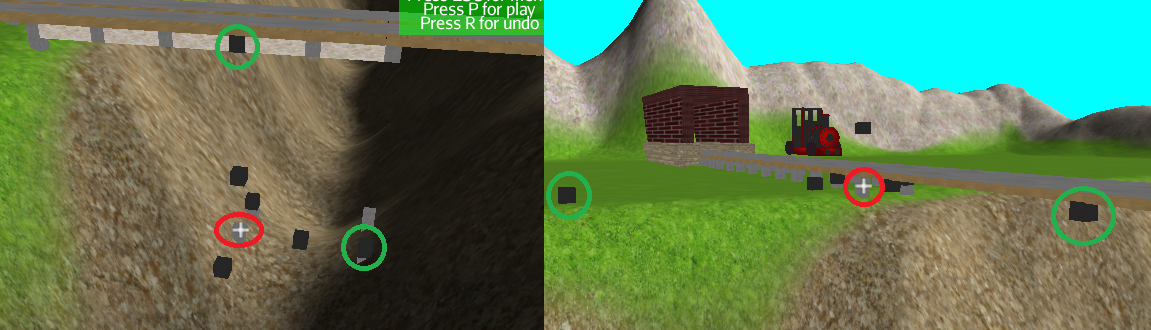
\includegraphics[width=1.0\textwidth]{screenshots/easyuse1.png}
    \caption{Empty world}
    \label{fig:easyu1}
\end{figure}
\begin{figure}[H]
    \centering
    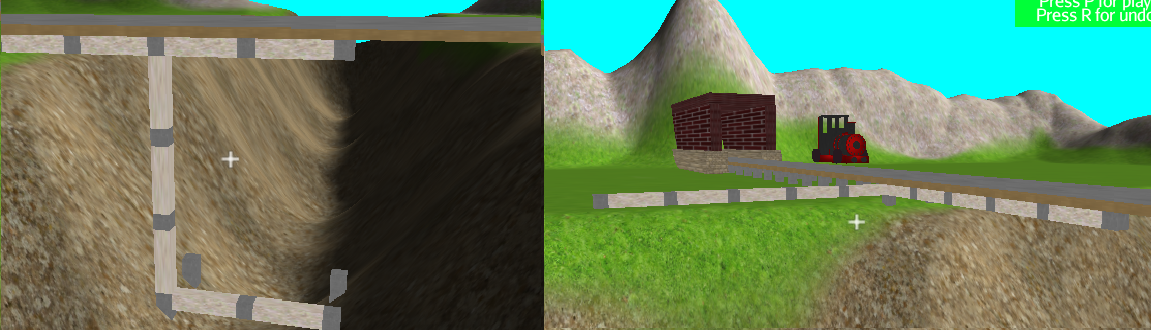
\includegraphics[width=1.0\textwidth]{screenshots/easyuse2.png}
    \caption{Empty world}
    \label{fig:easyu2}
\end{figure}
\subsubsection{Sample run}
When you start a new level, there will be an empty world as shown in \ref{fig:startup}. There will be connection points on both sides of the ravine. Depending on the level there could be more starting connection points. The user can start building a bridge by selecting a building block and a connection point. 
\begin{figure}[H]
    \centering
    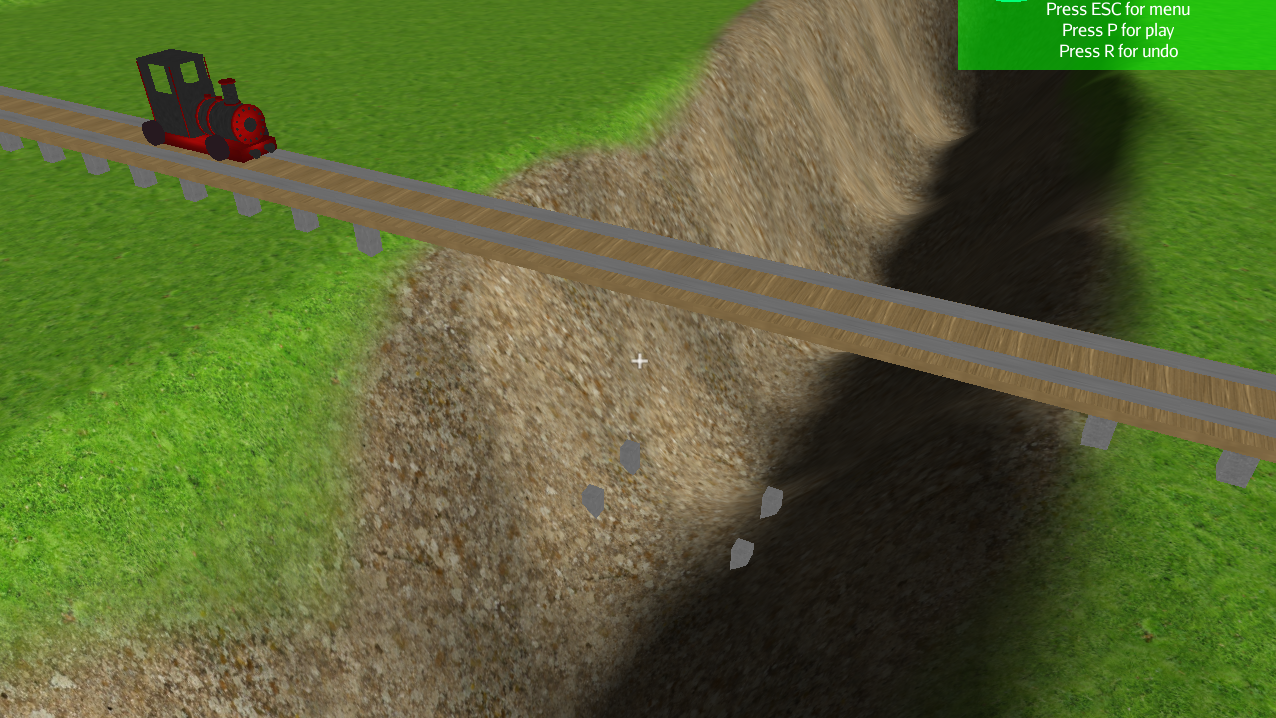
\includegraphics[width=0.8\textwidth]{screenshots/initial.png}
    \caption{Empty world}
    \label{fig:startup}
\end{figure}
After building a bridge the user can click on play, to start the simulation. The user cannot start the simulation if the 4 connection points are not connected. There has to be a connection between both sides of the ravine. A bridge built correctly is shown in \ref{fig:fullbridge}.
\begin{figure}[H]
    \centering
    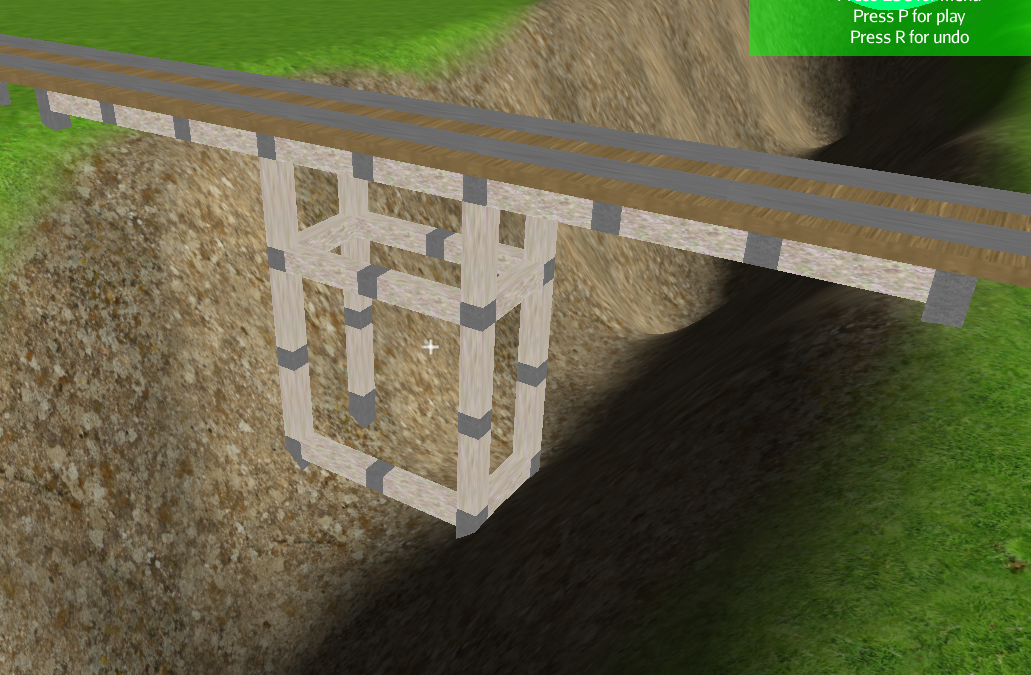
\includegraphics[width=0.8\textwidth]{screenshots/fullbridge.png}
    \caption{Bridge}
    \label{fig:fullbridge}
\end{figure}
When the user clicked on play and the bridge is built correctly, there will be a rail added automatically to the bridge. A train will ride over the bridge and the bridge will collapse or the train gets to the other side of the ravine safely as show in \ref{fig:full}
\begin{figure}[H]
    \centering
    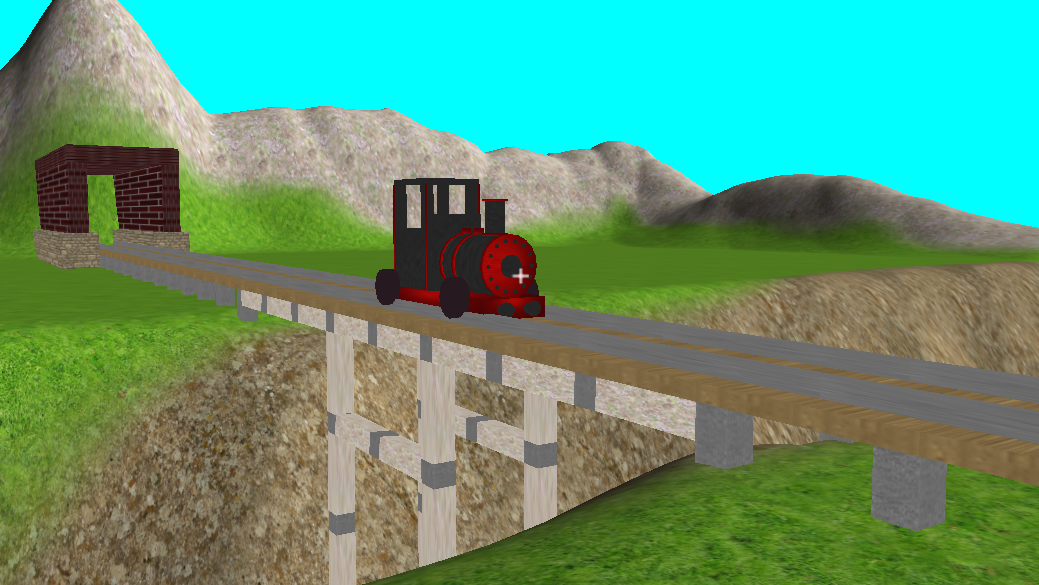
\includegraphics[width=0.8\textwidth]{screenshots/Drives.png}
    \caption{Succeed!}
    \label{fig:full}
\end{figure}
\subsection{Evaluation}
\subsubsection{Known limitations}
The rail for over the bridge is already drawn, which makes it harder to build under the bridge. This makes it also possible to build through the rails, which causes the physic engine to behave unrealistic. This is shown in \ref{fig:limit1}
\begin{figure}[H]
    \centering
    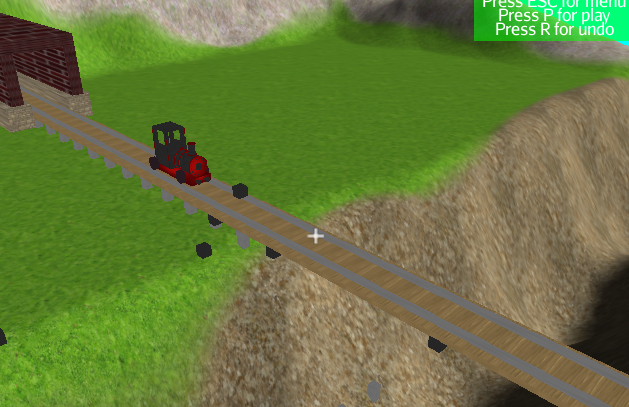
\includegraphics[width=0.4\textwidth]{screenshots/limit1.png}
    \caption{Building under the bridge is hard}
    \label{fig:limit1}
\end{figure}
When building, the block to which you want to build is black. This can be hard to see sometimes as the background can be a bit dark too. This is shown in \ref{fig:limit2}
\begin{figure}[H]
    \centering
    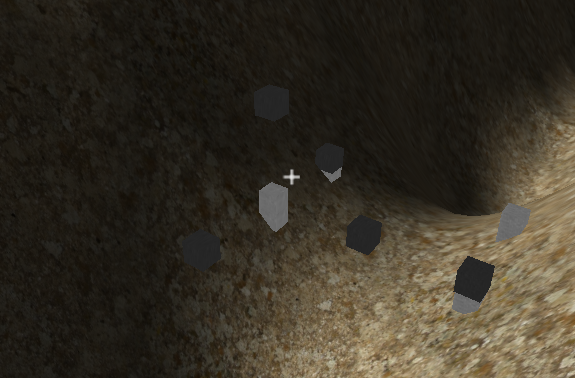
\includegraphics[width=0.4\textwidth]{screenshots/limi2.png}
    \caption{Sometimes connection points are hard to see, because of a dark background}
    \label{fig:limit2}
\end{figure}
There also other things that could be improved, but these are discussed in the next section.